\documentclass{article}
\usepackage{graphicx} % Required for inserting images
\usepackage{float}
\usepackage{hyperref}
\usepackage[italian]{babel}
\usepackage[a4paper, margin=2.5cm]{geometry}

\title{\textbf{CineMax - Manuale Utente}}
\author{Niccolò Jacopo Alt, Mateo Soldo, Davide Vignati}
\date{12/06/2026 v1.0}
\newpage
\begin{document}
\newpage

\maketitle
\newpage
\tableofcontents
\newpage

\section{Introduzione}
CineMax è un’applicazione software sviluppata in linguaggio Java per la gestione di un cinema monosala.  Il sistema è stato progettato nell’ambito del corso di Laboratorio Interdisciplinare A con l’obiettivo di realizzare una piattaforma in grado di gestire varie tipologie di utenti, proiezioni cinematografiche e prenotazioni.
\subsection{Funzionamento generale dell'applicazione}
L’applicazione permette ai clienti di registrarsi, effettuare il login, consultare le proiezioni disponibili e prenotare posti in sala.  
Gli operatori di biglietteria e i proiezionisti possono invece gestire le proiezioni, controllare le prenotazioni e amministrare i dati del sistema.
I dati vengono memorizzati tramite file CSV e gestiti attraverso le strutture dati messe a disposizione dal Java Collections Framework.  
Il progetto è stato sviluppato seguendo i principi della programmazione orientata agli oggetti, con particolare attenzione alla modularità, alla leggibilità del codice e alla separazione delle responsabilità tra le classi.

\section{Installazione}
\subsection{Requisiti di sistema}
Per eseguire l’applicazione è necessario predisporre l’ambiente installando Java JDK 21 (?) o superiore. (non so se mettere Maven anche nel manuale utente o solo nel tecnico).
I sistemi operativi supportati sono:
\begin{itemize}
    \item Windows (10 e 11)
    \item MacOs (Apple Silicon)
    \item Linux
\end{itemize}
NOTA: l’applicazione è stata sviluppata e testata in ambiente Windows 10/11 e MacOS 26; non è garantito il corretto funzionamento su piattaforma Linux. 

\subsection{Setup Ambiente}
Per l’utilizzo dell’applicazione è necessario disporre di un ambiente di esecuzione compatibile con Java. L’applicazione richiede la presenza del Java Runtime Environment (JRE), che consente l’esecuzione di programmi java senza la necessità di strumenti di sviluppo. Java Foundation (Oracle) distribuisce solo il JDK, che comprende anche il JRE, ecco come installarlo:



\subsubsection{JDK - Java development kit}
Per installare il JDK è necessario collegarsi sul sito Oracle e sotto la voce “Java Download” si troverà l’installazione che più si addice al sistema del computer. Si consiglia di scaricare la versione più recente e aggiornata che si trova a disposizione (in questo momento, JDK 26).

\begin{figure}[H]
    \centering
    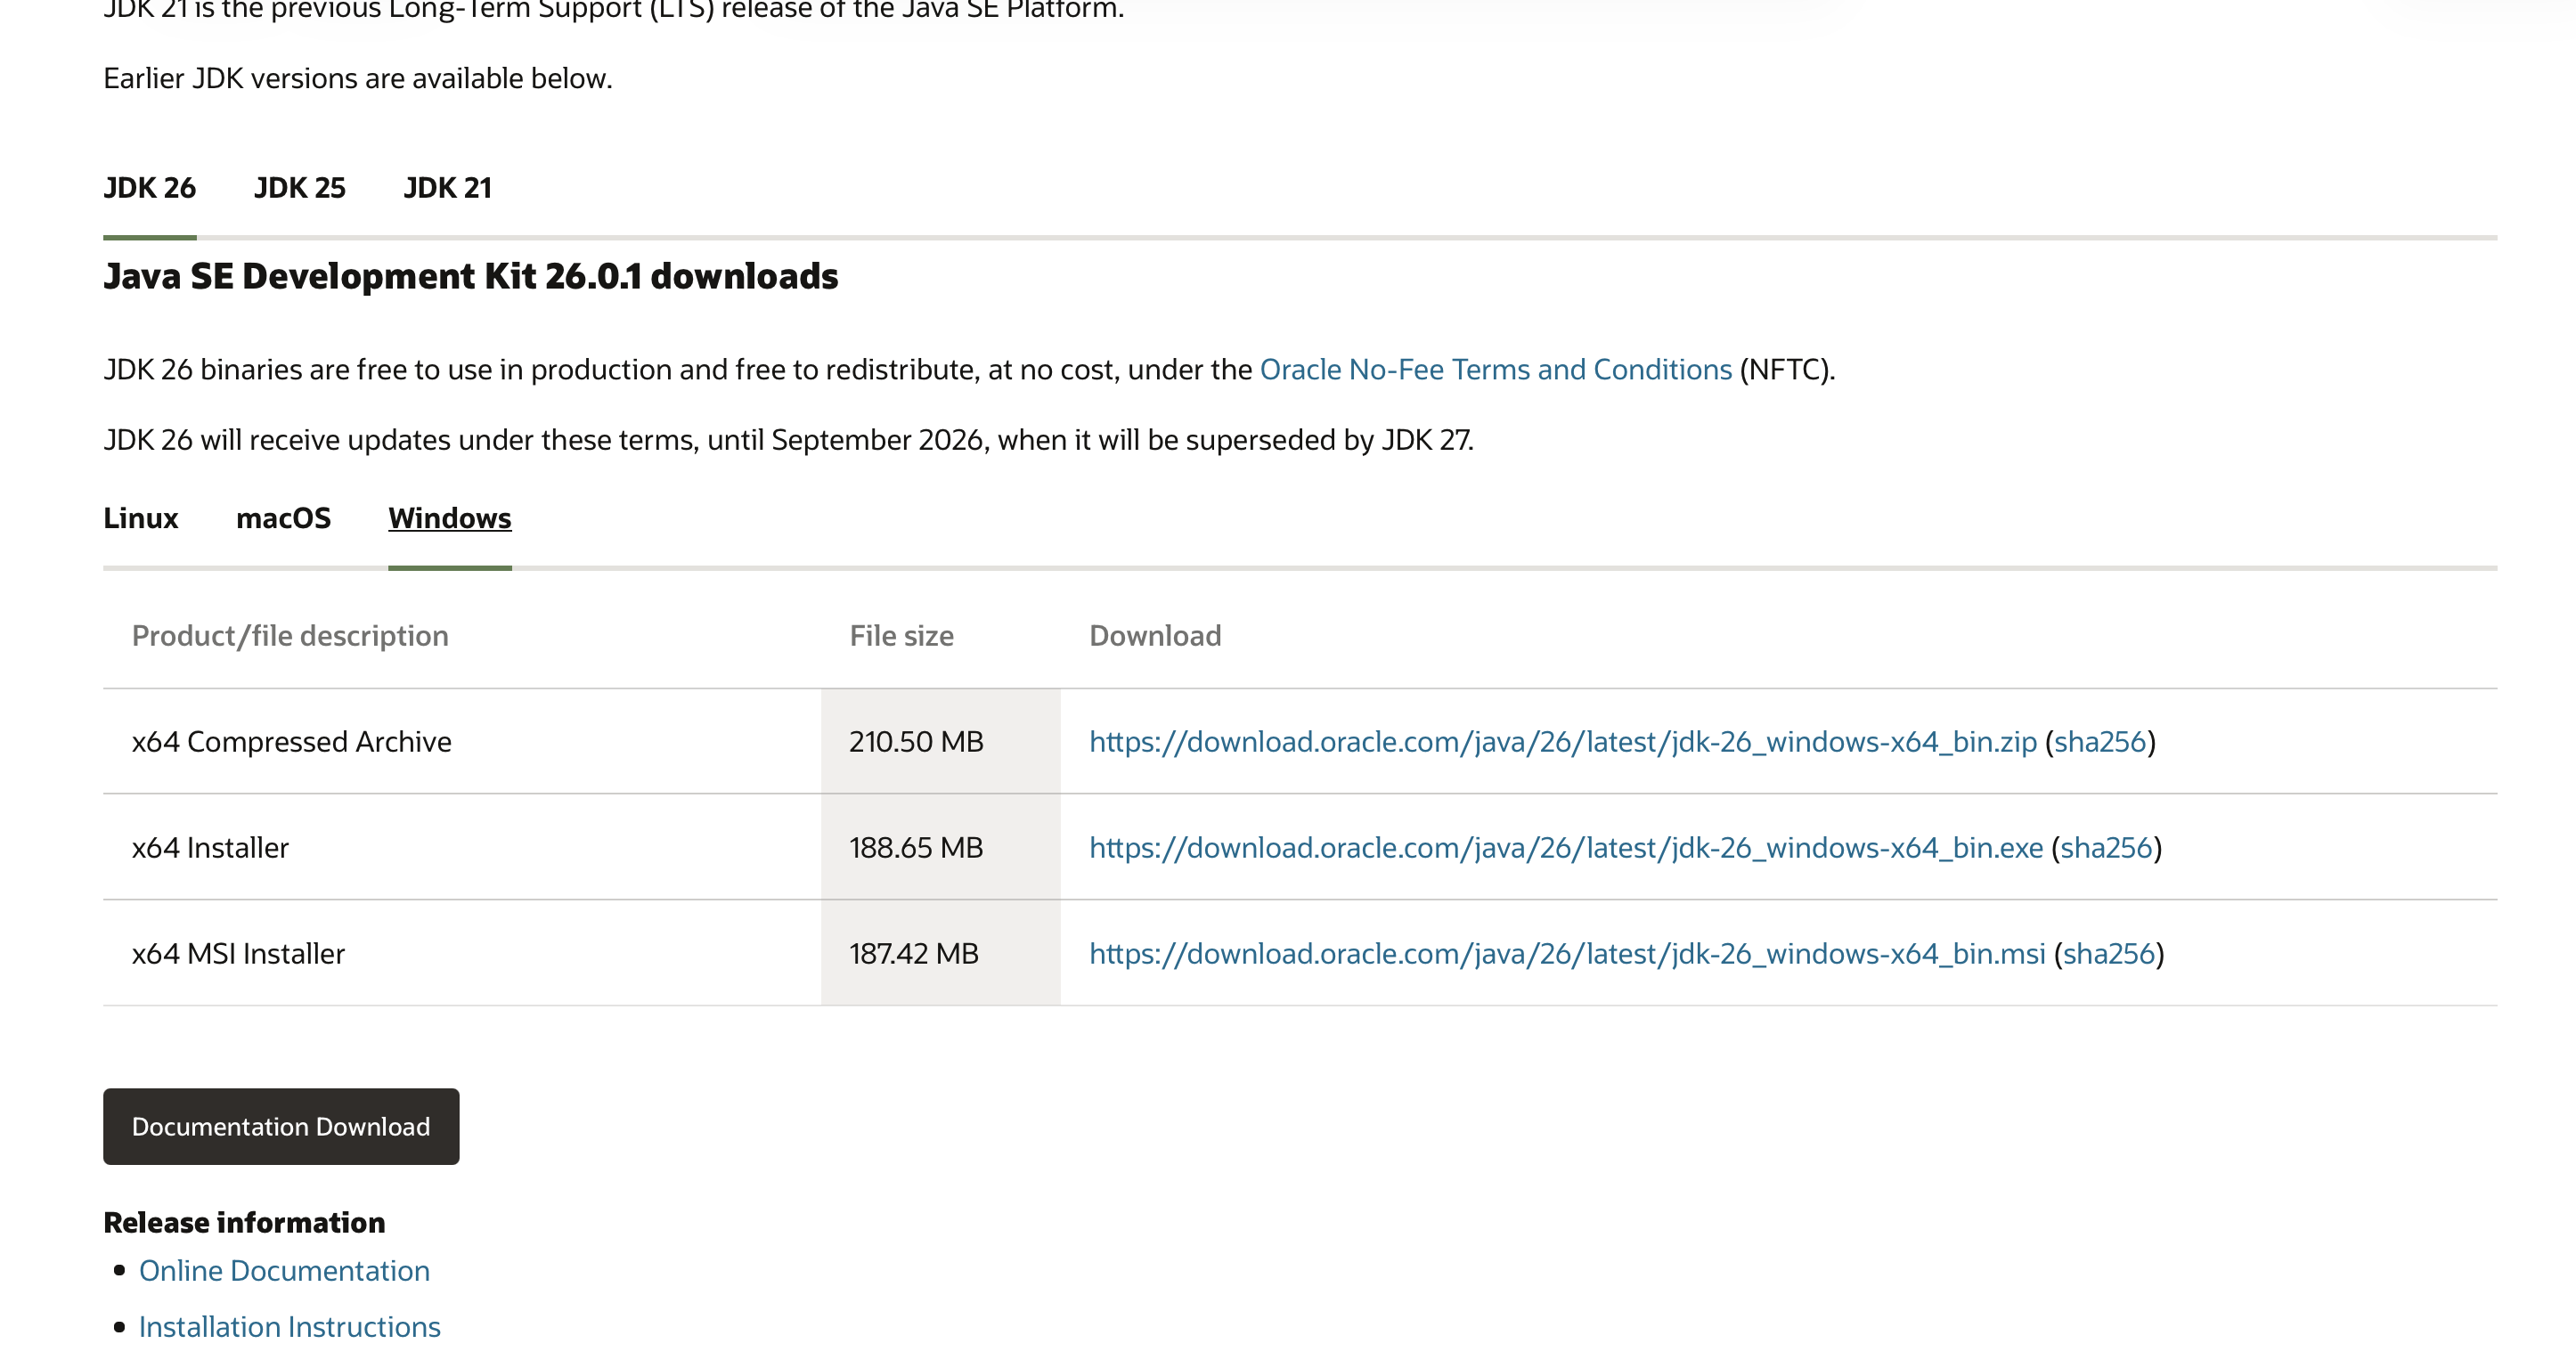
\includegraphics[width=0.9\linewidth]{pics/oracle.png}
    \label{fig:oracle}
\end{figure}

Una volta installato il JRE, l’applicazione può essere avviata eseguendo il file fornito con estensione .jar
\subsection{Installazione programma}
Per poter eseguire l’applicazione è necessario, inoltre, scaricare il software eseguibile all’interno del proprio dispositivo procedendo come indicato di seguito:

\begin{itemize}
    \item Fare clic per scaricare la cartella compressa
    \item Fare clic con il tasto destro sull’elemento con estensione “.zip” e selezionare la voce “Estrai i file…” quindi selezionare il percorso desiderato.
\end{itemize}

\section{Esecuzione ed uso}
\subsection{Avviare l'applicazione}
In base al sistema operativo utilizzato procedere con le seguenti istruzioni: per avviare l'applicazione con Windows e MacOS è sufficiente utilizzare la console dei comandi:
\begin{itemize}
    \item spostarsi sul percorso dove avete scaricato il file .jar tramite i comandi del terminale \textit{cd[percorso]}
    \item digitare java -jar bin/CineMax.jar; \textbf{Importante:}  esegui il comando dalla root del progetto.
\end{itemize}

\subsection{Uso delle funzionalità}
Le funzionalità disponibili all’interno dell’applicazione variano in base al tipo di utente che accede al sistema. In particolare, l’applicazione distingue tra diversi profili utente (clienti, proiezionisti e bigliettai), ciascuno dei quali dispone di permessi e funzionalità specifiche. Di seguito vengono descritte le operazioni che possono essere effettuate in base alla tipologia di utente:

\begin{figure}[H]
    \centering
    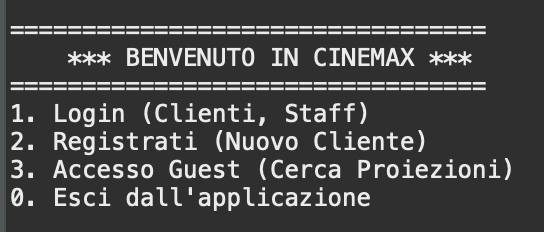
\includegraphics[width=0.7\linewidth]{pics/menu_principale.png}
    \label{fig:menu1}
\end{figure}

\subsubsection{Ospite (Guest) }
L’utente che utilizza l’applicazione senza effettuare l’accesso
\begin{itemize}
    \item Cercare le proiezioni;
    \item Visualizzare i dettagli delle proiezioni inserendo vari criteri di ricerca (titolo, genere, data, costo del biglietto);
	\item Effettuare la registrazione al servizio come Cliente inserendo          alcune informazioni personali e la scelta di un username e password;
	\item Effettuare l’accesso (login) al servizio come cliente inserendo le proprie credenziali;
\end{itemize}

\begin{figure}[H]
    \centering
    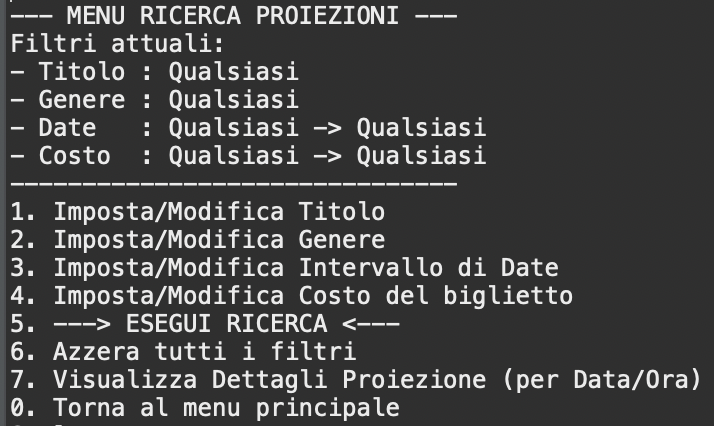
\includegraphics[width=0.7\linewidth]{pics/menu_guest.png}
    \label{fig:placeholder}
\end{figure}

\subsubsection{Cliente}
L’utente registrato che accede all’applicazione con le proprie credenziali.
\begin{itemize}
    \item Effettuare una nuova prenotazione andando a specificare data e ora della proiezione;
	\item Visualizzare le proprie prenotazioni;
	\item Modificare e cancellare le proprie prenotazioni;
\end{itemize}

\begin{figure}[H]
    \centering
    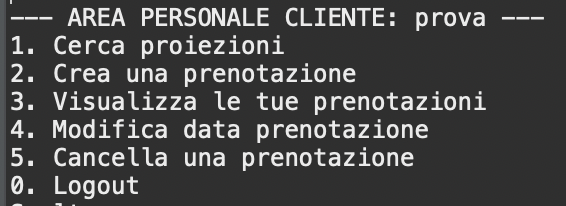
\includegraphics[width=0.7\linewidth]{pics/menu_cliente.png}
    \label{fig:menu2}
\end{figure}

\subsubsection{Proiezionista (staff)}
\begin{itemize}
    \item Inserire una nuova proiezione nel palinsesto andando a specificare anche il costo del biglietto per ogni proiezione
	\item Modificare la data di una proiezione senza prenotazioni
	\item Eliminare una proieizone

\end{itemize}
\subsubsection{Bigliettaio (staff)}
\begin{itemize}
    \item Visualizzare le prenotazione della giornata
	\item Cercare una prenotazione utilizzando diversi criteri di ricerca (Codice prenotazione, nome e cognome del cliente, titolo del film oppure per intervallo di date)
\end{itemize}

\subsection{Dataset di test}
Per verificare il corretto funzionamento dell'applicazione è stato utilizzato un dataset di test composto da dati di esempio, appositamente creati per simulare un utilizzo reale del sistema, come il file proiezioni.csv e utenti.csv. Il dataset di test è stato progettato per:
\begin{itemize}
    \item verificare la corretta lettura dei dati dai file CSV
    \item testare le funzionalità di visualizzazione, ricerca e filtraggio
    \item controllare il comportamento dell'applicazione in caso di inserimento di nuovi dati
\end{itemize}

\section{Limiti della soluzione sviluppata}

\begin{itemize}
    \item Gestione utenti limitata: L’applicazione non è concorrenziale, non è prevista la gestione di più utenti contemporaneamente.
\end{itemize}


\begin{itemize}
    \item Persistenza dei dati limitata: i dati possono essere memorizzati localmente o in modo non persistente, senza l’utilizzo di un database distribuito o remoto.
\end{itemize}

\begin{itemize}
    \item Interfaccia utente assente: l'applicazione è stata progettata per essere usata da terminale senza una vera e propria UI
\end{itemize}


\section{Sitografia / Bibliografia}
\url{https://www.oracle.com/it/java/technologies/downloads/}
altro da mettere?

\end{document}
